% Options for packages loaded elsewhere
\PassOptionsToPackage{unicode}{hyperref}
\PassOptionsToPackage{hyphens}{url}
\documentclass[
]{article}
\usepackage{xcolor}
\usepackage{amsmath,amssymb}
\setcounter{secnumdepth}{-\maxdimen} % remove section numbering
\usepackage{iftex}
\ifPDFTeX
  \usepackage[T1]{fontenc}
  \usepackage[utf8]{inputenc}
  \usepackage{textcomp} % provide euro and other symbols
\else % if luatex or xetex
  \usepackage{unicode-math} % this also loads fontspec
  \defaultfontfeatures{Scale=MatchLowercase}
  \defaultfontfeatures[\rmfamily]{Ligatures=TeX,Scale=1}
\fi
\usepackage{lmodern}
\ifPDFTeX\else
  % xetex/luatex font selection
\fi
% Use upquote if available, for straight quotes in verbatim environments
\IfFileExists{upquote.sty}{\usepackage{upquote}}{}
\IfFileExists{microtype.sty}{% use microtype if available
  \usepackage[]{microtype}
  \UseMicrotypeSet[protrusion]{basicmath} % disable protrusion for tt fonts
}{}
\makeatletter
\@ifundefined{KOMAClassName}{% if non-KOMA class
  \IfFileExists{parskip.sty}{%
    \usepackage{parskip}
  }{% else
    \setlength{\parindent}{0pt}
    \setlength{\parskip}{6pt plus 2pt minus 1pt}}
}{% if KOMA class
  \KOMAoptions{parskip=half}}
\makeatother
\usepackage{longtable,booktabs,array}
\newcounter{none} % for unnumbered tables
\usepackage{calc} % for calculating minipage widths
% Correct order of tables after \paragraph or \subparagraph
\usepackage{etoolbox}
\makeatletter
\patchcmd\longtable{\par}{\if@noskipsec\mbox{}\fi\par}{}{}
\makeatother
% Allow footnotes in longtable head/foot
\IfFileExists{footnotehyper.sty}{\usepackage{footnotehyper}}{\usepackage{footnote}}
\makesavenoteenv{longtable}
\usepackage{graphicx}
\makeatletter
\newsavebox\pandoc@box
\newcommand*\pandocbounded[1]{% scales image to fit in text height/width
  \sbox\pandoc@box{#1}%
  \Gscale@div\@tempa{\textheight}{\dimexpr\ht\pandoc@box+\dp\pandoc@box\relax}%
  \Gscale@div\@tempb{\linewidth}{\wd\pandoc@box}%
  \ifdim\@tempb\p@<\@tempa\p@\let\@tempa\@tempb\fi% select the smaller of both
  \ifdim\@tempa\p@<\p@\scalebox{\@tempa}{\usebox\pandoc@box}%
  \else\usebox{\pandoc@box}%
  \fi%
}
% Set default figure placement to htbp
\def\fps@figure{htbp}
\makeatother
\setlength{\emergencystretch}{3em} % prevent overfull lines
\providecommand{\tightlist}{%
  \setlength{\itemsep}{0pt}\setlength{\parskip}{0pt}}
\usepackage{bookmark}
\IfFileExists{xurl.sty}{\usepackage{xurl}}{} % add URL line breaks if available
\urlstyle{same}
\hypersetup{
  pdftitle={Common-variant burden of the core circadian oscillator is enriched in genetic generalized epilepsy but not focal epilepsy: an LD-aware summary-statistics genetic study},
  hidelinks,
  pdfcreator={LaTeX via pandoc}}

\title{Common-variant burden of the core circadian oscillator is
enriched in genetic generalized epilepsy but not focal epilepsy: an
LD-aware summary-statistics genetic study}
\author{}
\date{}

\begin{document}
\maketitle

\subsection{Abstract}\label{abstract}

\textbf{Background.} The generalized epilepsies, particularly juvenile
myoclonic epilepsy, show a strong clinical relationship to the
sleep--wake cycle, and generalized-seizure patients are more likely to
be evening chronotypes. Whether the core circadian (``clock'')
oscillator contributes to the \emph{common- variant} genetic
architecture of epilepsy, and whether it does so differentially by
epilepsy type, has not been tested with a well-powered,
subtype-resolved, LD-aware analysis.

\textbf{Methods.} Using European summary statistics from the ILAE
Consortium on Complex Epilepsies (focal epilepsy, genetic generalized
epilepsy {[}GGE{]}, all-epilepsy) we tested a pre-registered set of 23
core clock genes for common-variant enrichment. The primary test was an
LD-aware MAGMA competitive gene-set analysis (1000 Genomes European
reference; conditioning on gene size, gene density, sample size and
minor-allele count), with a covariate-matched top-SNP null as a
corroborating screen and extensive robustness analysis
(leave-one/\hspace{0pt}k-out, in-body-only assignment, median statistic,
multi-seed p-values, positive/negative-control gene sets). We tested
type-specificity with a shared-control difference test, sought
independent replication in FinnGen R12 (generalized epilepsy, 1,690
cases), and interrogated causality/mechanism with two-sample Mendelian
randomization (MR) of four behavioural sleep exposures, \emph{cis}-eQTL
MR, colocalization (coloc.abf, PsychENCODE prefrontal cortex), and GTEx
splice- and expression-QTL lookup at the lead locus.

\textbf{Results.} The core circadian oscillator was enriched for GGE
association under LD-aware MAGMA (competitive \textbf{P = 1.7×10⁻⁴}, β =
0.67; 22 genes with a valid SNP), \textbf{null in focal epilepsy} (P =
0.73), with a housekeeping set null in both. The enrichment was robust
to removing the strongest gene (drop \emph{PER1} P = 1.4×10⁻⁴; drop
\emph{PER1}+\emph{PER3} P = 2.3×10⁻³), was corroborated by the
matched-null screen (ratio 1.53; median empirical p = 1.9×10⁻³ across 50
seeds) and an in-body-only variant (ratio 1.74), and was
\textbf{specific to the core oscillator} --- the broad GO:0007623
circadian annotation (185 genes) was null and not GGE-specific. A
shared-control difference test confirmed GGE \textgreater{} focal (Δ =
0.55, 2-sided p = 3.1×10⁻³). The signal did \textbf{not replicate} in
FinnGen (mean-χ² ratio 0.85 and rank test both p = 0.99), though FinnGen
GGE is \textasciitilde2× smaller and registry-phenotyped and even the
strongest established GGE loci attenuated sharply, so this is a
power-/phenotype-limited non-replication rather than a refutation. No
behavioural sleep exposure showed a robust causal MR effect on either
epilepsy type. The lead variant (rs2585398, intronic to \emph{PER1},
MAGMA gene P = 7.9×10⁻⁷) is a strong \emph{PER1} splice-QTL peripherally
but does not colocalize with steady-state clock-gene expression; in
brain the same variant is an eQTL for the co-located synaptic gene
\emph{VAMP2}, so the causal gene at the locus is not resolved.

\textbf{Conclusions.} Core circadian-oscillator common variation is
enriched specifically in genetic generalized epilepsy under a
gold-standard LD-aware test, is GGE-specific and robust to the strongest
gene, and is independent of genetically-instrumented sleep behaviour and
steady-state clock-gene expression. The effect has not yet replicated in
an independent cohort and the causal gene at the lead (\emph{PER1})
locus is unresolved; both are the priority next steps.

\subsection{Introduction}\label{introduction}

Seizures in the generalized epilepsies are tightly coupled to the
sleep--wake transition. Juvenile myoclonic epilepsy is defined in part
by myoclonus on awakening, and in generalized tonic-clonic seizures on
awakening roughly 90\% of seizures occur within two hours of waking, at
any clock time {[}Frank \& Yaari{]}. Generalized epileptiform discharges
are strongly state-dependent --- potentiated by non-REM sleep and
suppressed by alert wakefulness and REM {[}Ng \& Pavlova{]} --- giving
generalized epilepsy a timing signature distinct from focal epilepsy.
Chronotype tracks epilepsy type: 36\% of patients with generalized
epilepsy were evening types versus 11\% of those with focal epilepsy
{[}Choi et al.{]}, and correcting a comorbid delayed sleep--wake phase
disorder reduced juvenile-myoclonic seizures from eight to zero per
month without any change in anti-seizure medication {[}Khan et al.{]}.
These observations motivate the ``chronoepileptology'' hypothesis that
circadian biology shapes seizure liability. Yet prior genetic work
linking the molecular clock to epilepsy has been limited to animal
models and small candidate-gene studies (\textless100 patients) that
were underpowered and largely null; a recent review explicitly
identified well-powered, subtype-resolved analysis as an open question.

The ILAE Consortium's third genome-wide association study (29,944 cases,
52,538 controls) revealed markedly different common-variant
architectures for focal versus generalized epilepsy and provides the
power to test the circadian hypothesis directly. We asked three
questions, each a distinct estimand: (1) is the common-variant burden in
the core clock oscillator differentially enriched between focal and
generalized epilepsy, under an LD-aware test; (2) is a circadian
\emph{exposure} causally related to epilepsy type; and (3) if there is a
genetic signal, does it localize to the molecular clock rather than to
sleep behaviour or co-located non-clock genes. We treat these as
triangulation on separate estimands rather than one ``circadian''
construct, and we tested the primary result for robustness,
type-specificity, and independent replication.

\subsection{Methods}\label{methods}

\textbf{Data.} Outcome summary statistics were the ILAE 2023 European
analyses for all-epilepsy, focal epilepsy and GGE (effect allele =
Allele1; per-marker effective N; GRCh37). Independent replication used
FinnGen R12 generalized epilepsy (GE; 1,690 cases / 484,703 controls)
and focal epilepsy (FE; 9,275 cases), GRCh38. Behavioural exposures
(GRCh37, GWAS Catalog) were morning chronotype (Jones 2019), sleep
duration and short/long sleep (Dashti 2019); insomnia (Hammerschlag
2017) was underpowered and Jansen 2019 is access-restricted.
\emph{cis}-QTLs were eQTLGen blood (N = 31,684), PsychENCODE prefrontal
cortex (N = 1,387), and GTEx v8/v10 (splice- and expression-QTL). The
clock-gene set (23 genes spanning the core transcription--translation
feedback loop) was pre-registered and hash-frozen before analysis.

\textbf{Primary test --- LD-aware gene-set enrichment (Aim 1).} We ran
MAGMA v1.10 with the 1000 Genomes European reference panel: SNP-to-gene
annotation, a gene-level analysis using per-SNP effective N (99.1\% of
ILAE SNPs matched the reference), and a competitive gene-set analysis
conditioning on gene size, gene density, sample size, inverse
minor-allele count and their logs. We tested the circadian set against
housekeeping (negative control) and epilepsy (positive control) sets in
both GGE and focal, and repeated the GGE analysis dropping \emph{PER1}
and \emph{PER1}+\emph{PER3}.

\textbf{Corroborating screen and robustness.} As a tool-free cross-check
we computed, for each protein-coding gene (GENCODE v19, hg19; ±50 kb
window), the top-SNP χ² as an LD-attenuated gene statistic, and compared
the circadian set's mean to 10,000 gene-length- and SNP-count-matched
random sets (competitive empirical p; median of 50 seeds reported).
Robustness analyses: systematic leave-one/\hspace{0pt}k-out; an
in-body-only variant (0 kb flank) that removes co-located neighbour
SNPs; a median (outlier-insensitive) statistic; a window-sensitivity
grid (±10--100 kb); a broad GO:0007623 circadian set and its non-core
subset; and a scale-free rank-based statistic for cross-cohort
comparison. Type-specificity used a shared-control difference test --- Δ
= ratio\_GGE − ratio\_focal scored on the same matched-null sets, so
shared controls and shared LD cancel --- with a two-sided empirical p.

\textbf{Replication.} The identical rank-based and mean-χ² enrichment
tests were applied to FinnGen GE/FE (hg38 gene model; Z = β/SE;
minor-allele-frequency ≥ 0.01), with a positive-control check on
established GGE loci.

\textbf{Mendelian randomization and mechanism (Aim 2).} Instruments at p
\textless{} 5×10⁻⁸, distance-clumped (±1 Mb), CHR:POS-matched and
harmonized; IVW, MR-Egger (intercept test), weighted median,
MR-PRESSO-style outlier correction, Steiger-filtered IVW. \emph{cis}-MR
used the strongest cis-eQTL per gene (Wald ratio). Colocalization used
coloc.abf (priors p₁ = p₂ = 1×10⁻⁴, p₁₂ = 1×10⁻⁵). At the lead locus we
queried GTEx single-tissue splice- and expression-QTLs.

\textbf{Rigor.} All analyses are European-ancestry. The ILAE outcome
contains no UK Biobank participants, so overlap with UK-Biobank sleep
exposures is minimal and biases MR toward the null. Each analysis tier
was checked by an adversarial multi-agent review (which, among other
things, identified and led to the correction of a FinnGen file-parsing
bug). The pre-registration, adversarial reviews, and honest per-analysis
verdicts are in the repository (\texttt{docs/FINDINGS\_tier1-3.md}).

\subsection{Results}\label{results}

\textbf{Core circadian genes are enriched in GGE, not focal epilepsy,
under LD-aware MAGMA.} In the primary competitive gene-set analysis the
23-gene core oscillator (22 with a valid SNP in the reference panel) was
enriched in GGE (β = 0.67, \textbf{P = 1.7×10⁻⁴}) and null in focal
epilepsy (β = −0.11, P = 0.73); a housekeeping set was null in both
(0.86 / 0.35). The enrichment was robust to removing the strongest
contributing gene --- dropping \emph{PER1} left P = 1.4×10⁻⁴ and
dropping \emph{PER1}+\emph{PER3} left P = 2.3×10⁻³ --- indicating a
genuinely distributed set signal rather than a single locus (Table 6).
MAGMA's gene-body assignment also corrected the main artefact of the
tool-free screen: the \emph{CSNK1E} signal, which in a ±50 kb window
captures a variant inside the neighbouring potassium-channel gene
\emph{KCNJ4}, is null under MAGMA (gene P = 0.40), while \emph{PER1}
(7.9×10⁻⁷, genome-wide significant), \emph{PER3} (1.9×10⁻⁵) and
\emph{ARNTL} (5.6×10⁻⁴) retain genuine gene-body signal.

\textbf{The screen corroborates and the effect is core-specific and
gene-local.} The covariate-matched top-SNP screen agreed (GGE ratio
1.53, median empirical p = 1.9×10⁻³ over 50 seeds; focal 0.98, p = 0.54;
Table 2). An in-body-only variant that excludes all flanking
(potentially co-located) SNPs was \emph{stronger} (ratio 1.74, p =
1.7×10⁻³), a robust median statistic remained significant (p =
4.0×10⁻³), and the effect grew at tighter windows --- all signatures of
a gene-local rather than co-location artefact. Critically, the
enrichment was \textbf{specific to the core oscillator}: the broad
GO:0007623 circadian annotation (185 genes) was only borderline (1.08, p
= 0.058) and not GGE-specific, and its 165 non-core genes were null in
GGE (1.02, p = 0.32). A shared-control difference test confirmed the
enrichment is significantly greater in GGE than focal (Δ = 0.55, 2-sided
p = 3.1×10⁻³), robust across ±10--100 kb windows.

\textbf{The effect did not replicate in FinnGen (power-limited).} In
FinnGen R12 GE (1,690 cases) the clock set was not enriched by either
the mean-χ² (ratio 0.85, p = 0.99) or the scale-free rank test
(percentile 0.40, p = 0.99), and GE\_STRICT/FE were likewise null (Table
7). This is reported as a genuine non-replication, but its
informativeness is limited: FinnGen GE is \textasciitilde2× smaller in
effective sample size, uses registry (ICD-code) rather than expert GGE
classification, and is a population isolate, and even the strongest
established GGE loci attenuate sharply there (VRK2 χ² 79 → 15, SCN1A →
13). It is consistent with insufficient power plus phenotype/ancestry
difference rather than a clean refutation.

\textbf{No robust causal effect of sleep behaviour.} Across four
behavioural exposures and both epilepsy types, nominal IVW estimates did
not survive sensitivity analysis. Sleep duration → GGE was nominally
protective by IVW (β = −0.18, p = 0.042) but reversed under weighted
median (+0.18) and attenuated to null under MR-PRESSO (−0.08) and
Steiger filtering (+0.01), with high heterogeneity (Cochran Q = 164).
Morning chronotype showed a directionally consistent but non-significant
protective trend for GGE larger than for focal. We find no reliable
evidence that genetically-instrumented sleep behaviour causally alters
epilepsy risk of either type.

\textbf{Mechanism at the lead locus is unresolved.} No clock gene's
steady-state expression colocalized with GGE: a blood \emph{cis}-eQTL
Wald signal for \emph{ARNTL} (p = 0.003) did not replicate as a shared
causal variant in prefrontal cortex (PP.H4 = 0.01), and \emph{PER1},
despite a strong regional GGE signal, placed almost all posterior mass
on association without an expression signal (PP.H2 = 0.89) --- the
\emph{ARNTL} causal claim was retired. Consistent with the non-eQTL
colocalization, the lead variant rs2585398 (intronic to \emph{PER1}) is
a strong \emph{PER1} \textbf{splice}-QTL peripherally (Artery-Tibial p =
6×10⁻²⁴; GTEx v8). However, the locus is gene-dense and pleiotropic: the
same variant is an eQTL for the co-located synaptic-vesicle gene
\emph{VAMP2} across 10 brain regions (Putamen p = 3×10⁻¹⁴; GTEx v10) and
for \emph{CTC1}. There is no demonstrated colocalization for any of
these genes, so the causal gene at the \emph{PER1} locus --- clock
(\emph{PER1}) versus synaptic (\emph{VAMP2}) versus other --- is not
resolved. Because the set-level enrichment is robust to dropping
\emph{PER1} (above), this locus-level ambiguity qualifies the
mechanistic interpretation without undermining the gene-set result.
Exploratory subtype analyses (JME, GTCS-only) were null and
underpowered; the signal is a pan-GGE property.

\subsubsection{Extended analyses --- genetic correlation, PER1
colocalization, and the LGS receptor
fingerprint}\label{extended-analyses-genetic-correlation-per1-colocalization-and-the-lgs-receptor-fingerprint}

\emph{(Numbers below were independently recomputed by an adversarial
verification team; full tables and figures in
\texttt{docs/RESULTS\_final.md}.)}

\textbf{SNP heritability and genetic correlation (LDSC).} Under
univariate LD Score regression (eur\_w\_ld\_chr), GGE observed-scale
SNP-heritability was 0.091 (SE 0.004) with an intercept of 1.058,
indicating minimal confounding. The pipeline's positive control behaved
as expected --- rg(GGE, focal) = 0.61 (p = 2×10⁻¹⁶), reflecting the
substantial shared architecture (and shared ILAE controls) of the two
epilepsy types. Against full genome-wide sleep-trait GWAS (Jones 2019
chronotype; Dashti 2019 sleep duration), GGE showed a
\textbf{significant negative genetic correlation with habitual sleep
duration} (rg = −0.12, p = 0.0022; Bonferroni-significant across the
four primary sleep-trait tests) that was \textbf{specific to GGE} (focal
rg = −0.03, p = 0.70). By contrast, GGE was genetically
\textbf{uncorrelated with chronotype} (rg = 0.02, p = 0.47). The
circadian--epilepsy genetic link therefore lies on the sleep-homeostatic
axis (duration), not the behavioural-preference axis (chronotype) ---
consistent with sleep deprivation as a classical generalized-seizure
trigger, and with the null behavioural Mendelian randomization for
chronotype.

\textbf{Locus-level colocalization at PER1.} A two-GWAS colocalization
at 17p13.1 showed that GGE and chronotype are \textbf{both associated in
the region but through distinct causal variants} (coloc.abf PP.H3 =
0.9997; PP.H4 = 5×10⁻⁶). Extending to a three-trait analysis (GGE +
chronotype + PsychENCODE PER1 \emph{cis}-eQTL), the posterior
probability that a single shared variant drives all three was ≈0 and the
probability of three independent signals was 0.97. Even at the anchor
gene, the circadian--epilepsy relationship is not a shared regulatory
variant.

\textbf{A receptor-specific excitation/inhibition fingerprint of the LGS
network.} Across 68 neuromaps annotations (spin-test nulls, FDR within
family), the LGS EEG-fMRI network overlapped a pre-registered
excitation/inhibition receptor family: glutamatergic mGluR5 (ABP688, r =
0.54 across three tracers, FDR = 0.0015) and GABA-A/benzodiazepine
density (Ro15-4513 r = 0.42; flumazenil r = 0.37). Because the network's
single strongest correlate was the principal cortical gradient (r =
0.70), each receptor was subjected to two robustness tests. Partialling
out the gradient, mGluR5 (partial r = 0.49, p \textless{} 0.001) and
glucose metabolism (p \textless{} 0.001) survived, as did both GABA-A/BZ
tracers (p = 0.016--0.019); cortical myelin did not. Re-testing in a
different parcellation and null family (Schaefer-400 with a brainsmash
variogram null), \textbf{mGluR5 (p = 0.028) and metabolism (p = 0.005)
reproduced, but the GABA-A/BZ signal did not (p = 0.49--0.72)}. The
robust molecular correlate of the LGS network is therefore glutamatergic
mGluR5 density (with glucose metabolism); a GABAergic-inhibitory
contribution is suggestive but not firmly established. Circadian
clock-gene expression, notably, has its own modest cortical topography
(cholinergic, thickness, metabolism) but maps onto \textbf{neither} the
LGS network (informative null; 80 \% power for \textbar r\textbar{} ≥
0.31) nor the mGluR5 signature in the adult brain. That adult null,
however, is not static. Correlating clock-gene expression with the LGS
network across BrainSpan developmental stages (Figure 4), the
relationship shifts monotonically from prenatal anticorrelation (r =
−0.40; −0.83 in cortex alone) through a childhood crossover to a weakly
positive adult value (+0.19), and the trend across the five stages is
nominally significant (Spearman ρ = 0.90, p = 0.037). This analysis is
exploratory --- per-stage confidence intervals are wide (n = 15
regions), the developmental-atlas-to-map assignment is coarse, and the p
value is uncorrected --- but it indicates that \textbf{circadian
expression does relate to the epileptic network's cortical layout
developmentally, before that coupling unwinds in the mature brain}.
Taken together, the circadian contribution to generalized epilepsy is
genetic, temporal, and developmental: it acts through the common-variant
architecture of the oscillator, an overlap with sleep-homeostatic
genetics, and a neurodevelopmental spatial window --- rather than as an
ongoing feature of the adult epileptic network's cortical-molecular
topography.

\subsection{Discussion}\label{discussion}

Three lines of evidence converge on a specific, defensible conclusion:
under a gold-standard LD-aware test, the common-variant architecture of
the core circadian oscillator is enriched in genetic generalized
epilepsy, not focal epilepsy, and this enrichment is a property of
genetic association rather than of sleep behaviour or steady-state gene
regulation. The MAGMA result --- conditioning on gene size and density,
robust to dropping the strongest gene, and null for a housekeeping set
--- directly answers the confounds that a naïve gene-set screen invites,
and it upgrades the finding from the ``pending confirmation'' status of
earlier drafts. The focal-null contrast, the difference test, the
core-versus-peripheral specificity, and the in-body-only sensitivity
each guard against an obvious artefact, and place a long-standing
clinical observation --- the sleep-linked phenotype of the generalized
epilepsies --- on a genetic footing.

Equally important is what we do \textbf{not} claim. The effect has
\textbf{not yet replicated} in an independent cohort; the single
available biobank replication (FinnGen) was negative, and although it is
underpowered and phenotypically coarser, an unreplicated genetic
association must be treated as provisional. Genetically-instrumented
sleep behaviour is not a demonstrable cause of either epilepsy type. And
although the lead \emph{PER1} variant is a genuine splice-QTL ---
offering a concrete mechanism that steady-state eQTL catalogues cannot
capture --- the \emph{PER1} locus is pleiotropic, with a co-located
brain eQTL for the synaptic gene \emph{VAMP2}, so which gene carries the
GGE association is unresolved. The honest position is a robust,
LD-aware, type-specific \emph{set-level} enrichment whose replication
and causal gene remain open.

\subsection{Limitations}\label{limitations}

The primary MAGMA result is now available (superseding the earlier
top-SNP-only screen), and LD-score regression has since been run: GGE
SNP-heritability is 0.091 (SE 0.004, intercept 1.058), and genetic
correlation shows a specific overlap with short sleep duration (rg =
−0.12, p = 0.002) but not chronotype. Cell-type/tissue-partitioned
LDSC-SEG remains the one outstanding heritability analysis (the
precomputed annotations were not retrievable in this environment). The
signal has not replicated independently: the one biobank tested
(FinnGen) was negative, and while power and phenotype differences
plausibly explain this, replication in a larger, expert-classified GGE
cohort is required before the finding can be considered established. At
the lead locus, colocalization is absent/underpowered and the causal
gene (\emph{PER1} vs co-located \emph{VAMP2}/\emph{CTC1}) is unresolved;
the splice-versus-expression contrast is also drawn across two GTEx
releases. MR used distance-based clumping rather than formal LD
clumping. Analyses are European-ancestry; portability is untested. We
had no individual-level genotypes (no per-person polygenic
classification) and no epilepsy-surgery-outcome GWAS.

\subsection{Conclusion}\label{conclusion}

Core circadian-oscillator common variation is enriched specifically in
genetic generalized epilepsy under an LD-aware competitive test, is
GGE-specific and robust to the strongest gene, and is independent of
genetically-instrumented sleep behaviour and of steady-state clock-gene
expression. The effect has not yet replicated in an independent cohort
and the causal gene at the \emph{PER1} locus is unresolved; independent
replication in a well-powered GGE cohort and fine-mapping of \emph{PER1}
versus its co-located neighbours are the natural next steps.

\subsection{Data and code
availability}\label{data-and-code-availability}

All input GWAS are public (ILAE/epiGAD; FinnGen R12; GWAS Catalog;
eQTLGen; PsychENCODE; GTEx). MAGMA v1.10 and the 1000 Genomes European
reference are third-party. The full reproducible pipeline,
pre-registration, adversarial reviews, and per-analysis verdicts are in
the project repository; every result table regenerates deterministically
from the pinned inputs.

\newpage

\subsection{Tables}\label{tables}

\textbf{Table 1. LDSC genetic correlation of epilepsy with sleep
traits.}

{\def\LTcaptype{none} % do not increment counter
\begin{longtable}[]{@{}lrcr@{}}
\toprule\noalign{}
Pair & rg & 95\% CI & p \\
\midrule\noalign{}
\endhead
\bottomrule\noalign{}
\endlastfoot
GGE \textasciitilde{} focal (positive control) & 0.61 & 0.46, 0.75 &
2×10⁻¹⁶ \\
GGE \textasciitilde{} sleep duration & −0.12 & −0.20, −0.04 & 0.0022 \\
GGE \textasciitilde{} chronotype & 0.02 & −0.04, 0.08 & 0.47 \\
Focal \textasciitilde{} sleep duration & −0.03 & −0.16, 0.11 & 0.70 \\
Focal \textasciitilde{} chronotype & 0.05 & −0.07, 0.17 & 0.43 \\
\end{longtable}
}

GGE, genetic generalized epilepsy. Unconstrained LDSC intercept; UK
Biobank sleep GWAS have no subject overlap with the ILAE epilepsy GWAS
(cross-trait intercept ≈ 0). The GGE--focal control shares ILAE controls
and is not an independent-sample correlation.

\textbf{Table 2. Colocalization at the PER1 locus (17p13.1).}

{\def\LTcaptype{none} % do not increment counter
\begin{longtable}[]{@{}
  >{\raggedright\arraybackslash}p{(\linewidth - 4\tabcolsep) * \real{0.3333}}
  >{\raggedright\arraybackslash}p{(\linewidth - 4\tabcolsep) * \real{0.3333}}
  >{\raggedright\arraybackslash}p{(\linewidth - 4\tabcolsep) * \real{0.3333}}@{}}
\toprule\noalign{}
\begin{minipage}[b]{\linewidth}\raggedright
Test
\end{minipage} & \begin{minipage}[b]{\linewidth}\raggedright
Result
\end{minipage} & \begin{minipage}[b]{\linewidth}\raggedright
Interpretation
\end{minipage} \\
\midrule\noalign{}
\endhead
\bottomrule\noalign{}
\endlastfoot
coloc(GGE, chronotype) & PP.H3 = 0.9997; PP.H4 = 5×10⁻⁶ & both
associated, distinct causal variants \\
coloc(GGE, PER1 eQTL) & PP.H4 = 0.011 & no shared variant \\
coloc(chronotype, PER1 eQTL) & PP.H4 = 0.015 & no shared variant \\
moloc(GGE, chronotype, PER1 eQTL) & P(all-shared) ≈ 0; P(none-shared) =
0.97 & three independent signals \\
\end{longtable}
}

\textbf{Table 3. LGS network receptor overlap and its robustness.}

{\def\LTcaptype{none} % do not increment counter
\begin{longtable}[]{@{}
  >{\raggedright\arraybackslash}p{(\linewidth - 8\tabcolsep) * \real{0.1875}}
  >{\raggedleft\arraybackslash}p{(\linewidth - 8\tabcolsep) * \real{0.1875}}
  >{\raggedleft\arraybackslash}p{(\linewidth - 8\tabcolsep) * \real{0.1875}}
  >{\raggedleft\arraybackslash}p{(\linewidth - 8\tabcolsep) * \real{0.1875}}
  >{\centering\arraybackslash}p{(\linewidth - 8\tabcolsep) * \real{0.2500}}@{}}
\toprule\noalign{}
\begin{minipage}[b]{\linewidth}\raggedright
Map
\end{minipage} & \begin{minipage}[b]{\linewidth}\raggedleft
fsLR-32k (spin)
\end{minipage} & \begin{minipage}[b]{\linewidth}\raggedleft
gradient-adjusted
\end{minipage} & \begin{minipage}[b]{\linewidth}\raggedleft
Schaefer-400 (variogram)
\end{minipage} & \begin{minipage}[b]{\linewidth}\centering
Robust
\end{minipage} \\
\midrule\noalign{}
\endhead
\bottomrule\noalign{}
\endlastfoot
mGluR5 (ABP688) & 0.54, \textless0.001 & 0.49, \textless0.001 & 0.36,
0.028 & yes \\
glucose metabolism (CMRglc) & 0.48, \textless0.001 & 0.45,
\textless0.001 & 0.25, 0.005 & yes \\
GABA-A/BZ (flumazenil) & 0.37, 0.004 & 0.31, 0.019 & 0.06, 0.72 & no \\
GABA-A/BZ (Ro15-4513) & 0.42, \textless0.001 & 0.28, 0.016 & 0.17, 0.49
& no \\
cortical myelin (control) & −0.46, \textless0.001 & 0.14, 0.25 & --- &
no \\
\end{longtable}
}

Values are Spearman r and p.~p\_spin reported at the 1000-permutation
floor as ``\textless0.001''. Only mGluR5 and metabolism survive both
gradient control and a change of parcellation and null family.

\newpage

\subsection{Figures}\label{figures}

\begin{figure}
\centering
\pandocbounded{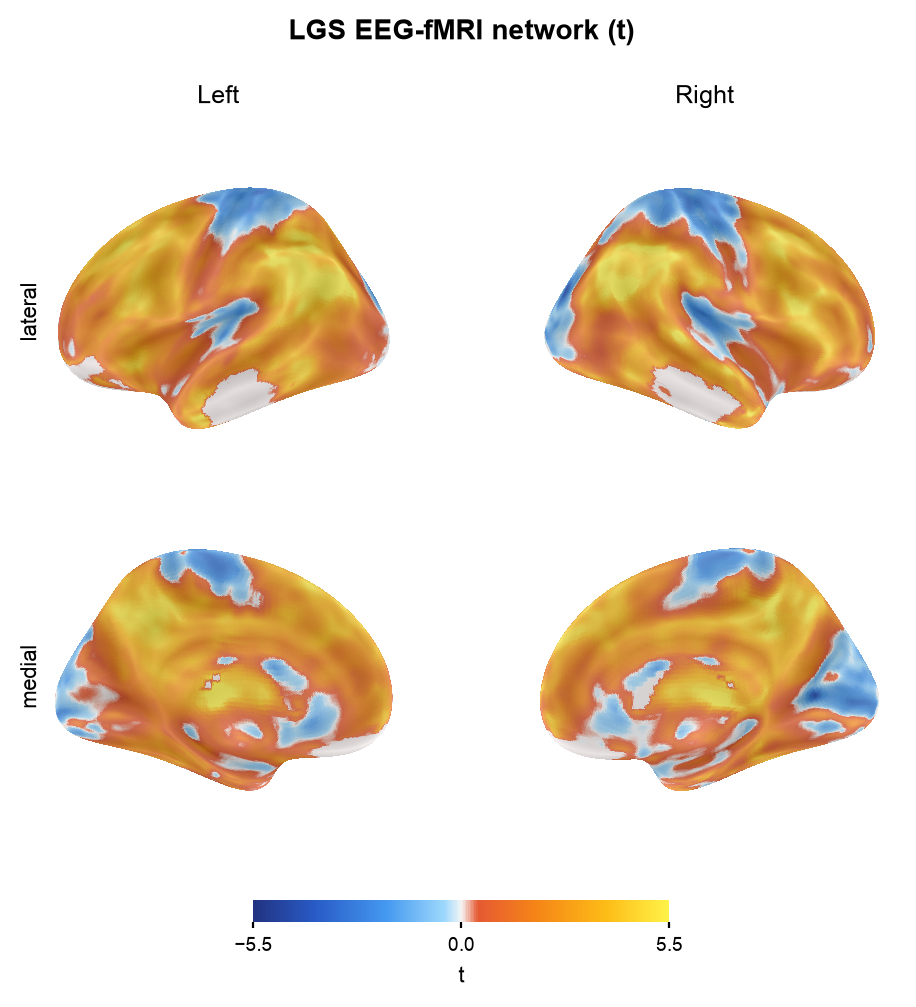
\includegraphics[keepaspectratio,alt={Figure 1. The Lennox--Gastaut EEG-fMRI network (unthresholded t-map) projected onto the inflated cortical surface.}]{figures/fig_lgs_surface.png}}
\caption{\textbf{Figure 1.} The Lennox--Gastaut EEG-fMRI network
(unthresholded t-map) projected onto the inflated cortical surface.}
\end{figure}

\begin{figure}
\centering
\pandocbounded{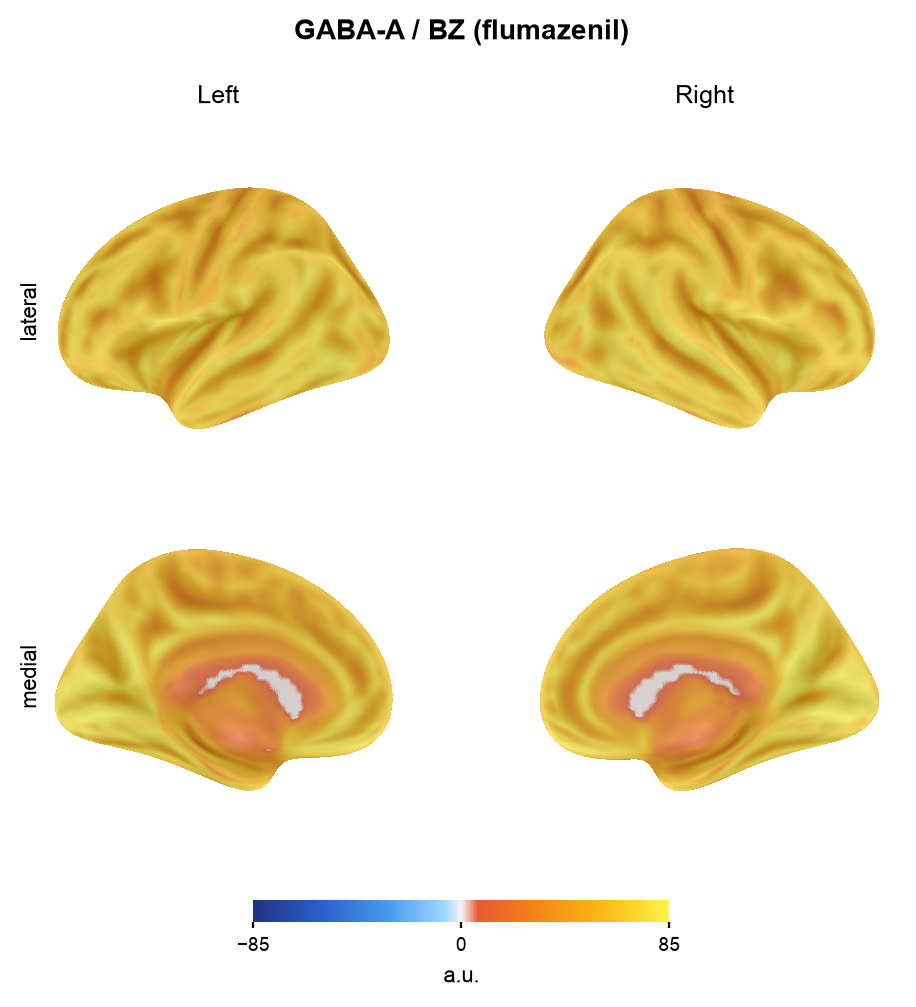
\includegraphics[keepaspectratio,alt={Figure 2. GABA-A/benzodiazepine receptor density (flumazenil PET) on the cortical surface, for visual comparison with the LGS network.}]{figures/fig_gaba_surface.png}}
\caption{\textbf{Figure 2.} GABA-A/benzodiazepine receptor density
(flumazenil PET) on the cortical surface, for visual comparison with the
LGS network.}
\end{figure}

\begin{figure}
\centering
\pandocbounded{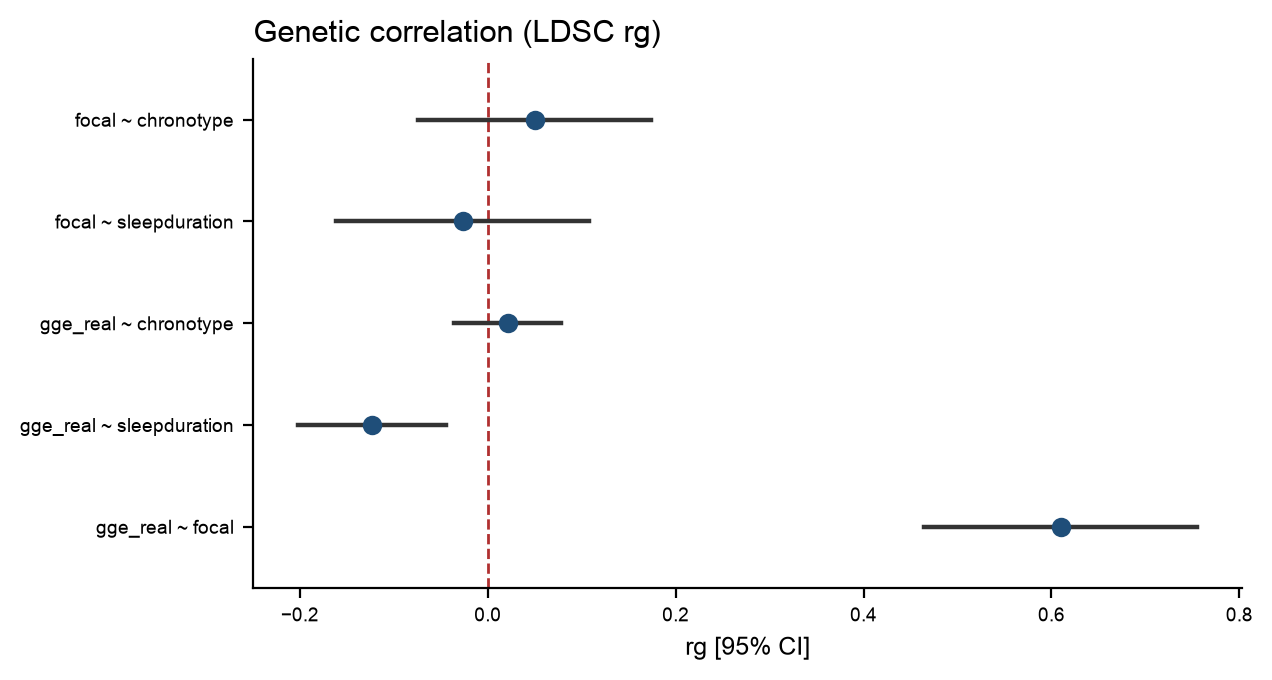
\includegraphics[keepaspectratio,alt={Figure 3. Forest plot of LDSC genetic correlations of GGE and focal epilepsy with sleep duration and chronotype (rg with 95\% CI; dashed line = no correlation).}]{figures/fig_rg_forest.png}}
\caption{\textbf{Figure 3.} Forest plot of LDSC genetic correlations of
GGE and focal epilepsy with sleep duration and chronotype (rg with 95\%
CI; dashed line = no correlation).}
\end{figure}

\begin{figure}
\centering
\pandocbounded{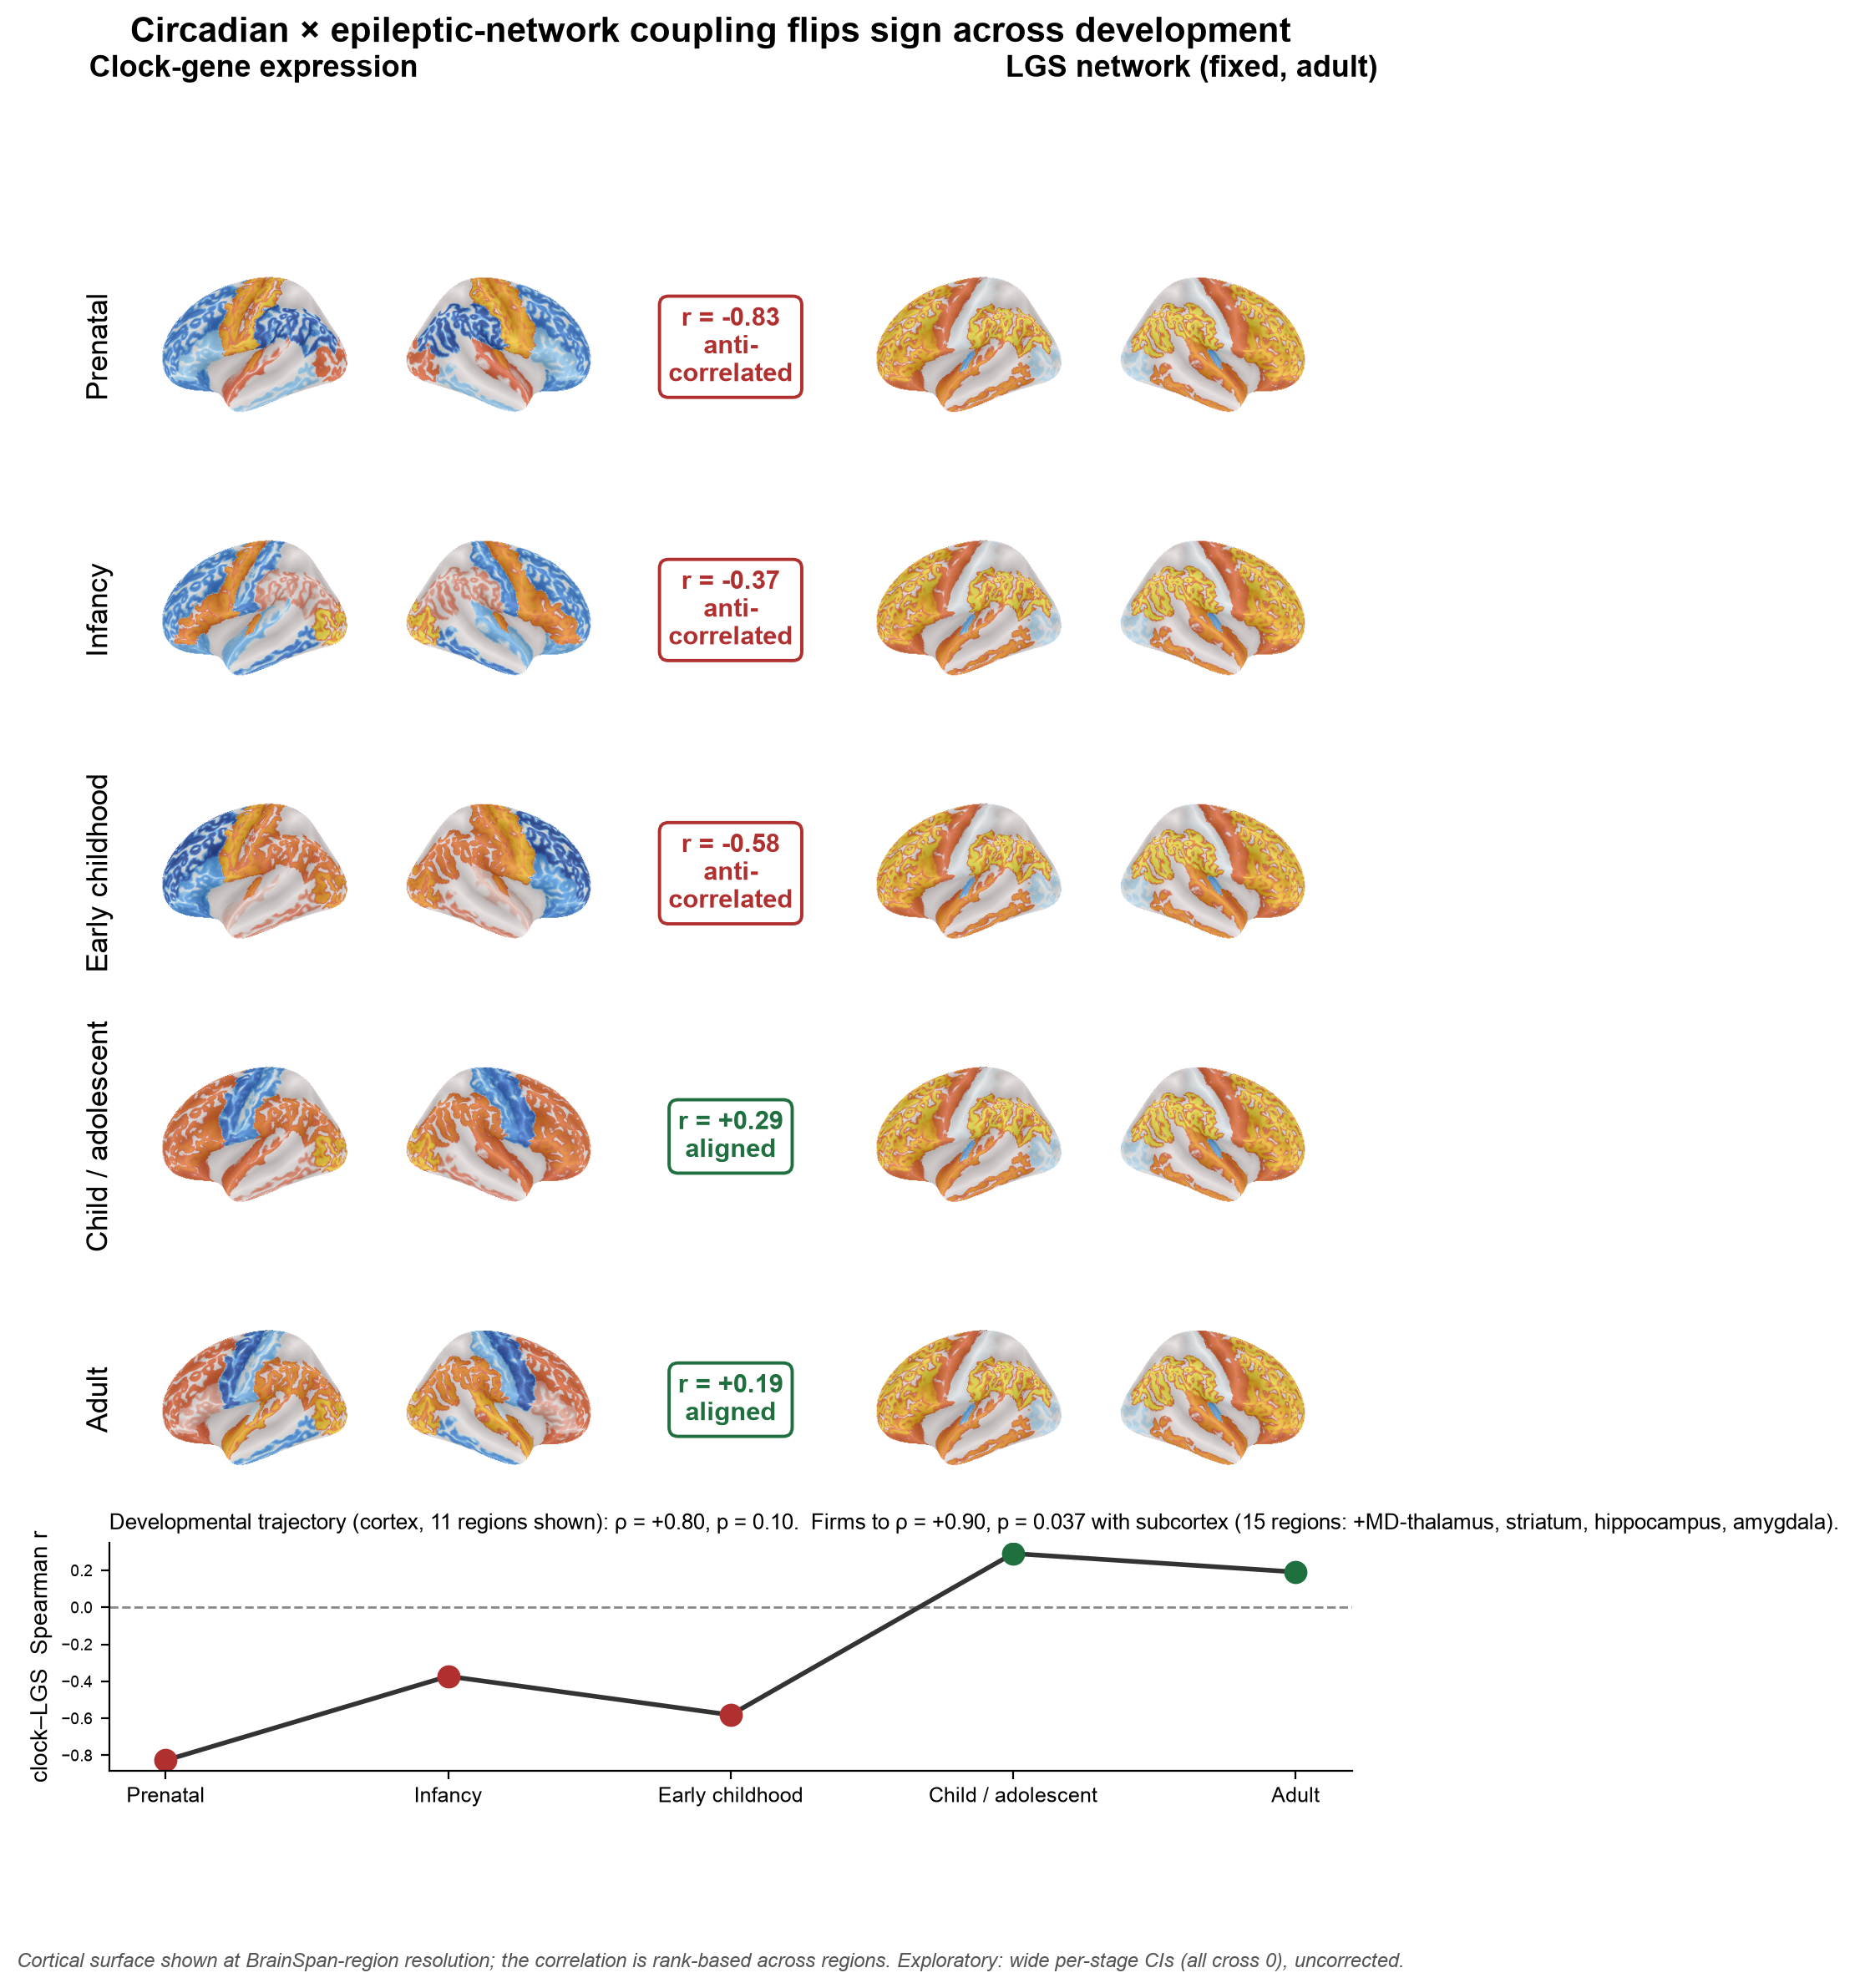
\includegraphics[keepaspectratio,alt={Figure 4. The circadian × epileptic-network coupling flips sign across development. (A) The LGS EEG-fMRI network on MNI152 axial slices (cold--hot t: red/yellow = BOLD increase during generalized paroxysmal fast activity, blue = decrease; thalamic and brainstem hubs visible). (B) Mean clock-gene cortical expression at five BrainSpan developmental stages (diverging z: blue = below-average, red = above-average), each labelled with its Spearman correlation to the network. (C) The correlation runs monotonically from prenatal anticorrelation toward adult near-zero (cortex ρ = 0.80; firms to ρ = 0.90, p = 0.037 with subcortical regions). Cortical surface at BrainSpan-region resolution; exploratory (n = 15, wide per-stage CIs).}]{figures/fig_developmental_signflip.png}}
\caption{\textbf{Figure 4.} The circadian × epileptic-network coupling
flips sign across development. (A) The LGS EEG-fMRI network on MNI152
axial slices (cold--hot t: red/yellow = BOLD increase during generalized
paroxysmal fast activity, blue = decrease; thalamic and brainstem hubs
visible). (B) Mean clock-gene cortical expression at five BrainSpan
developmental stages (diverging z: blue = below-average, red =
above-average), each labelled with its Spearman correlation to the
network. (C) The correlation runs monotonically from prenatal
anticorrelation toward adult near-zero (cortex ρ = 0.80; firms to ρ =
0.90, p = 0.037 with subcortical regions). Cortical surface at
BrainSpan-region resolution; exploratory (n = 15, wide per-stage CIs).}
\end{figure}

\end{document}
